\documentclass[a4paper]{article}

\usepackage[utf8]{inputenc}
\usepackage[portuges]{babel}
\usepackage{indentfirst}
\usepackage{graphicx}
\usepackage{float}
\usepackage{caption}
\usepackage{subcaption}
\usepackage[T1]{fontenc}
\usepackage{listings}
\usepackage{amsmath}
\usepackage{mathtools}
\renewcommand{\familydefault}{\sfdefault}


\title{Projeto de Computação Gráfica - Fase 2}
\author{Diogo Braga A82547 \and João Silva A82005 \and Ricardo Caçador A81064
\and Ricardo Veloso A81919}
\date{\today}

\begin{document}

\maketitle

\begin{abstract}
Neste relatório é apresentada a segunda fase dum projeto no qual a intenção é desenvolver um mecanismo baseado em gráficos 3D e fornecer exemplos de uso que mostrem o seu potencial. Este projeto é desenvolvido no âmbito da unidade curricular de Computação Gráfica.
\end{abstract}

\tableofcontents


\newpage

\section{Introdução}
\label{sec:intro}

Esta segunda fase tem como objetivo a realização de algumas etapas, nomeadamente:
\begin{enumerate}
\item A criação dum parser \emph{XML} mais conciso;
\item A alteração/evolução da estrutura dos ficheiros \emph{XML};
\item A criação de estruturas capazes de armazenar as figuras necessárias;
\item A criação de funções que leiam as estruturas e as desenhem;
\item A criação dum modelo estático do sistema solar.
\end{enumerate}

De seguida iremos apresentar todos os algoritmos e decisões relativos à realização destas etapas, bem como as respetivas explicações de cada passo.
Serão ainda apresentadas figuras e esquemas que ilustrem os passos do processo desenvolvido.



\section{Estrutura da Pasta do Projeto}
\label{sec:estrutura}

Para um entendimento mais claro da estrutura do projeto, achamos por bem referenciar a estrutura da pasta do projeto.
O projeto entregue contêm para além do relatório, 4 pastas como é possível verificar na seguinte figura.

\begin{figure}[H]
\centering
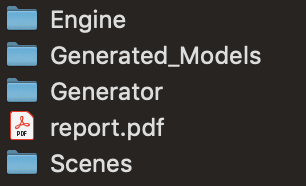
\includegraphics[scale=1.0]{estrutura.png}
\caption{Estrutura da pasta.}
\label{img:estrutura}
\end{figure}

Na pasta \textbf{Engine} residem os ficheiros relativos ao programa \emph{engine}, bem como as bibliotecas (.h) criadas para o efeito. Contém ainda um ficheiro de configuração \emph{cmake} e os ficheiros relativos à biblioteca \emph{tinyxml2}.

Na pasta \textbf{Generator} residem os ficheiros relativos ao programa \emph{generator}. Contém também um ficheiro de configuração \emph{cmake}.

Na pasta \textbf{Generated\_Models} residem os ficheiros que contêm os pontos gerados para cada figura, criados pelo programa \emph{generator}.

Na pasta \textbf{Scenes} residem os ficheiros \emph{XML} que contêm as estruturas do sistemas solares desenvolvidos para esta fase do projeto. Construímos dois ficheiros deste tipo, um que contém os raios relativos de cada planeta e do sol baseados na realidade (grande disparidade entre as figuras criadas), e o outro que é mais elucidativo e percetível.


\newpage

\section{Parser XML}
\label{sec:parser}

\subsection{Ficheiro}
\label{sec:ficheiro}

Devido aos requerimentos desta fase, foi necessário criar um novo ficheiro XML com o intuito de representar o sistema solar, que inclui: o sol, os planetas, e os satélites naturais destes mesmos.

Esta nova cena é encabeçada pelo grupo que faz referencia ao sol, e possui vários sub-grupos. Estes sub-grupos são referentes aos planetas, e possuem também sub-grupos. Estes sub-grupos dos planetas são referentes aos satélites naturais que cada um possui.

Todos os sub-grupos herdam as transformações geométricas presentes no grupo ao qual pertencem. Nesta fase, estas transformações são: translações, rotações e escalas.

Na figura \ref{img:ficheiro_parser} é possível visualizar um excerto do ficheiro XML por nós usado no qual constam o Sol, a Terra e a Lua.

\begin{figure}[H]
\centering
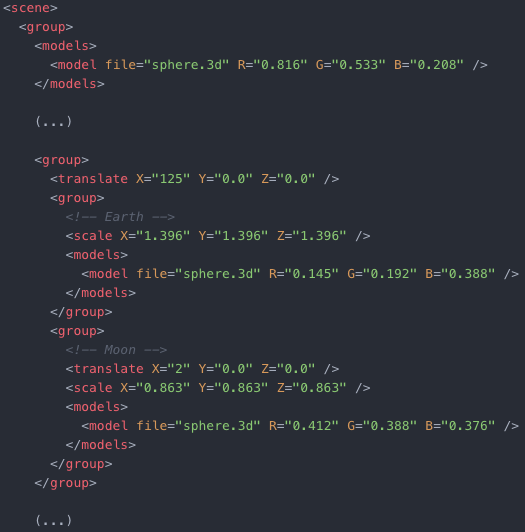
\includegraphics[scale=0.6]{ficheiro_parser.png}
\caption{Exemplo dum ficheiro usado no Parser.}
\label{img:ficheiro_parser}
\end{figure}

\subsection{Funcionamento}
\label{sec:funcionamento}


\newpage

\section{Estruturas de Dados}
\label{sec:estruturas}
Quanto à estrutura de dados, o grupo considerou que a mais adequado seria a de representar o sistema solar como uma árvore, sendo que, analogamente ao primeiro nodo da árvore estaria o Sol e os planetas seriam os \textit{filhos} do Sol nessa árvore. Em consequência, as luas seriam \textit{filhos} dos planetas e \textit{netos} do Sol.  Para esta representação ser efetiva foram criadas varias estruturas que serão apresentadas a seguir neste relatório.


\subsection{Tree}
\label{sec:tree}

A classe Tree será usada para representar uma Árvore. Uma instância de Árvore tem uma \textbf{Figure} principal e um \textbf{vector} com os \textit{filhos} que tem.

\begin{figure}[H]
\centering
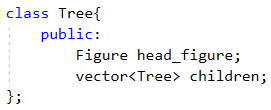
\includegraphics[scale=0.8]{tree.png}
\caption{Estrutura que define instâncias de uma Árvore}
\label{img:Tree}
\end{figure}


\subsection{Figure}
\label{sec:figure}

A classe Figure é composta por um inteiro com o número de triângulos que constitui essa figura, um vector com os pontos todos da figura. Possui também as 3 transformações geométricas que são feitas sobre a mesma - Translation, Rotation, Scale. Contém ainda uma Color, para definir a cor da figura.

\begin{figure}[H]
\centering
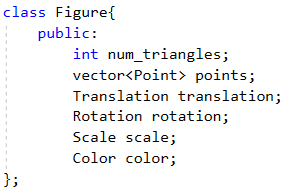
\includegraphics[scale=0.8]{figure.png}
\caption{Estrutura que define instâncias de uma Figura}
\label{img:Figure}
\end{figure}


\subsection{Color}
\label{sec:color}

A classe Color é composta por 3 floats - r,g e b. Estes floats juntos definem a cor para usar numa figura.

\begin{figure}[H]
\centering
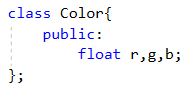
\includegraphics[scale=0.8]{color.png}
\caption{Estrutura que define instâncias de Cor.}
\label{img:Color}
\end{figure}


\subsection{Scale}
\label{sec:scale}

A classe Scale contém 3 floats - x,y e z, que são os parâmetros de redimensionamento da figura que queremos. Contém ainda um bool para verificar se a figura existe.

\begin{figure}[H]
\centering
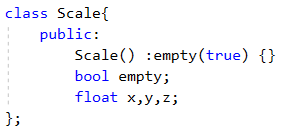
\includegraphics[scale=0.8]{scale.png}
\caption{Estrutura que define instâncias de Scale}
\label{img:Scale}
\end{figure}


\subsection{Rotation}
\label{sec:rotation}

A classe Rotation é composta por 4 floats - as coordenadas dos eixos e o ângulo que queremos rodar a figura. Tem também um bool empty que apenas permite a leitura caso o seu valor seja true.

\begin{figure}[H]
\centering
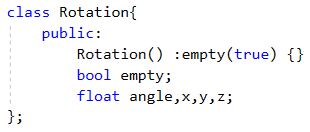
\includegraphics[scale=0.8]{rotation.png}
\caption{Estrutura que define instâncias de Rotation}
\label{img:Rotation}
\end{figure}


\subsection{Translation}
\label{sec:translation}

A classe Translation é também composta pelas 3 coordenadas dos eixos e pela verificação de que a figura existe mesmo e queremos lê-la.

\begin{figure}[H]
\centering
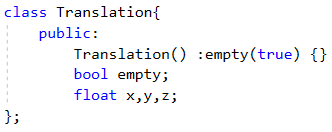
\includegraphics[scale=0.8]{translation.png}
\caption{Estrutura que define instâncias de Translation}
\label{img:Tree}
\end{figure}


\subsection{Point}
\label{sec:point}

A classe Point, como o nome indica, é um ponto no sistema, ou seja, é composta por 3 floats - x, y e z.

\begin{figure}[H]
\centering
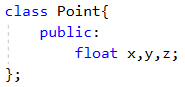
\includegraphics[scale=0.8]{point.png}
\caption{Estrutura que define instâncias de Point}
\label{img:Point}
\end{figure}


\newpage

\section{\textit{Render Scene}}

\newpage

\section{\textit{Upgrades da Fase Anterior}}

Em relação à fase anterior houve alguns pontos que foram sujeitos a mudanças e otimizações pelo que estas serão relatadas nesta secção.

Uma das partes que foi sujeita a otimização foi o cálculo das coordenadas da câmera que na fase anterior continha demasiado código e algumas variáveis que não tinham nexo em ser usadas.
Desta forma decidimos que esta parte deveria ser reescrita utilizando uma abordagem mais objetiva. O resultado é descrito na seguinte figura.

\begin{figure}[H]
\centering
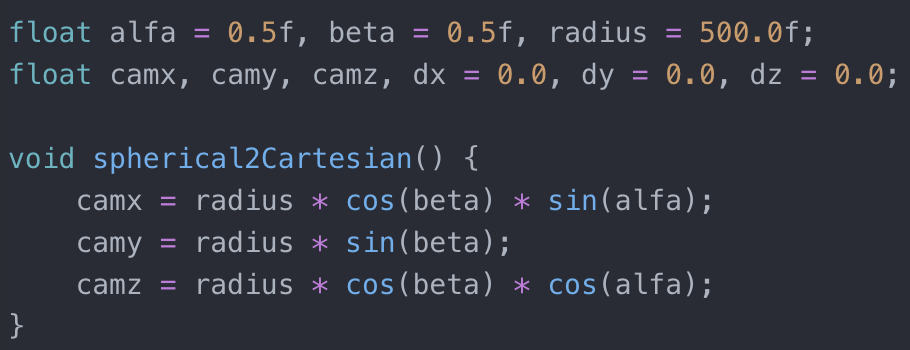
\includegraphics[scale=0.9]{camara.png}
\caption{Código referente às coordenadas da câmara.}
\label{img:camara}
\end{figure}

Não só a função que calcula as coordenadas para câmara mas também a própria função da câmara foi melhorada. Passou a poder mover-se consoante o ponto para o qual está a olhar. Desta forma possibilitou-nos a facilidade de podermos deslocarmo-nos para qualquer sítio que nos convenha. Tal alteração é descrita na seguinte figura.

\begin{figure}[H]
\centering
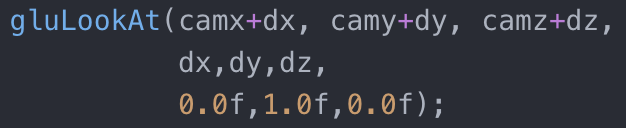
\includegraphics[scale=0.9]{mat_camara.png}
\caption{Função que contém a matriz da câmara.}
\label{img:mat_camara}
\end{figure}

!!!!!!!!!!!!!!!!!!!!!!!!!!!!!!!!!!!!!!!!! FALTA ACABAR !!!!!!!!!!!!!!!!!!!!!!!!!!!!!!!!!!!!!!!

FALAR DOS .H

\newpage

\section{Conclusão}
\label{sec:conclusao}

Após a conclusão desta fase do projeto, todos os membros do grupo se sentem mais à vontade com transformações geométricas e, consequentemente, com todos os conceitos apreendidos nas aulas que tiveram de ser colocados em prática nesta fase. Relativamente ao nível de execução desta fase o grupo no geral não sentiu grandes dificuldades, tendo apenas contado com um imprevisto, resolvido rapidamente que foi a dificuldade em *COMPLETAR COM A DIFICULDADE QUE TIVEMOS SÓ PARA ENCHER CHOURIÇOS E NÃO PARECER QUE SOMOS OS REIS DO CG*.
Em jeito de conclusão e revisão final a esta fase, o grupo espera continuar num bom caminho para a realização de todas as fases deste projeto, que, para já, tem sido um projeto prazeroso.

\section{Bibliografia}
\label{sec:bibliografia}

!!!!!!!!!!!!!!!!!!!!!!!!!!!!!!!!!!!!!!!!! POR FAZER !!!!!!!!!!!!!!!!!!!!!!!!!!!!!!!!!!!!!!!!!

https://www.suapesquisa.com/astronomia/distancia\_sol\_planetas.htm

\end{document}
